\documentclass[aspectratio=169,11pt]{beamer}

% Standard Beamer (Madrid) with a light-blue theme color.
\usetheme{Madrid}
\definecolor{ThemeBlue}{HTML}{5B9BD5}
\definecolor{ThemeDark}{HTML}{1F4E79}
\usecolortheme[named=ThemeBlue]{structure}
\setbeamercolor{alerted text}{fg=ThemeDark}
% Alerted text is also underlined; \uline (ulem) lets it break across lines.
\usepackage[normalem]{ulem}
\renewcommand<>{\alert}[1]{{\usebeamercolor[fg]{alerted text}\uline{#1}}}
\setbeamertemplate{navigation symbols}{}
\setbeamertemplate{itemize items}[circle]
\setbeamertemplate{enumerate items}[default]
\AtBeginSection[]{%
  \begin{frame}
    \vfill
    \centering
    \begin{beamercolorbox}[sep=10pt,center,rounded=true]{title}
      \usebeamerfont{title}\insertsectionhead
    \end{beamercolorbox}
    \vfill
  \end{frame}}
\setbeamerfont{footnote}{size=\tiny}

\usepackage{amsmath,amssymb,mathtools,bm}
\usepackage{booktabs,array}
\usepackage{fontawesome5}
\usepackage[most]{tcolorbox}
\usepackage{tikz}
\usetikzlibrary{positioning,calc,fit,shapes.misc}
\usepackage{listings}
\lstset{basicstyle=\ttfamily\scriptsize, columns=fullflexible, keepspaces=true,
  backgroundcolor=\color{ThemeBlue!12}, frame=none, breaklines=true}
\usepackage[backend=bibtex, style=numeric, sorting=none, maxbibnames=3,
  minbibnames=1, maxcitenames=1, mincitenames=1, giveninits=true, doi=false, url=false, isbn=false]{biblatex}
\addbibresource{references.bib}
\renewcommand*{\bibfont}{\tiny}

% Lecture numbers generated by the instructor's lecture-data scripts (not distributed); do not edit by hand.
\newcommand{\EightMaxScore}{378}
\newcommand{\EightMinScore}{160}
\newcommand{\EightRuntime}{1,508}
\newcommand{\GameLL}{1,511 / 1,506}
\newcommand{\GameLLserved}{A 70.4\,MW, B 70.3\,MW}
\newcommand{\GameLS}{2,759 / 1,601}
\newcommand{\GameLSserved}{92.2}
\newcommand{\GameNashText}{Nash equilibria: (A small, B large); (A large, B small).}
\newcommand{\GameSL}{1,601 / 2,580}
\newcommand{\GameSLserved}{89.1}
\newcommand{\GameSS}{1,601 / 1,601}
\newcommand{\HCabove}{146}
\newcommand{\HCbuses}{2,000}
\newcommand{\HCmedian}{372}
\newcommand{\HCmin}{10}
\newcommand{\HCpninety}{1,536}
\newcommand{\HCpoints}{48,000}
\newcommand{\HCpten}{130}
\newcommand{\HCruntime}{48,000 LPs in 549\,s}
\newcommand{\OrdBus}{7419}
\newcommand{\OrdHundred}{299}
\newcommand{\OrdHundredGain}{21}
\newcommand{\OrdTwentyFour}{274}
\newcommand{\OrdTwentyFourGain}{11}
\newcommand{\OrdZero}{248}
\newcommand{\PairHCa}{123}
\newcommand{\PairHCaGiven}{81}
\newcommand{\PairHCb}{135}
\newcommand{\SerOneBus}{1002}
\newcommand{\SerOneMax}{129}
\newcommand{\SerOneMed}{126}
\newcommand{\SerOneMin}{123}
\newcommand{\SerTwoBus}{7419}
\newcommand{\SerTwoMax}{699}
\newcommand{\SerTwoMed}{503}
\newcommand{\SerTwoMin}{248}
\newcommand{\StoB}{200}
\newcommand{\StoBig}{390}
\newcommand{\StoBus}{7419}
\newcommand{\StoHalfNo}{248}
\newcommand{\StoHalfWith}{298}
\newcommand{\StoMean}{390}
\newcommand{\StoMin}{248}
\newcommand{\StoP}{50}
\newcommand{\StoWith}{298}


\newcommand{\HC}{\ensuremath{\mathrm{HC}}}
\newcommand{\MW}{\ensuremath{\,\mathrm{MW}}}
\newcommand{\MWh}{\ensuremath{\,\mathrm{MWh}}}
% Decision variables of the hosting-capacity LP, each in its own color.
\definecolor{varL}{HTML}{C0392B}
\definecolor{varPg}{HTML}{0969DA}
\definecolor{varP}{HTML}{1A7F37}
\definecolor{varF}{HTML}{8250DF}
\newcommand{\vL}{{\color{varL}L}}
% Optional subscript, \vpg[t], so it stacks under the superscript g.
\NewDocumentCommand{\vpg}{o}{{\color{varPg}\IfValueTF{#1}{\mathbf{p}^{\mathrm{g}}_{#1}}{\mathbf{p}^{\mathrm{g}}}}}
\newcommand{\vp}{{\color{varP}\mathbf{p}}}
\newcommand{\vf}{{\color{varF}\mathbf{f}}}
\definecolor{varU}{HTML}{D35400}
\definecolor{varE}{HTML}{117A8B}
\newcommand{\vu}{{\color{varU}u}}
\newcommand{\ve}{{\color{varE}e}}
\definecolor{varG}{HTML}{B8860B}
\definecolor{varD}{HTML}{6D4C41}
\newcommand{\vg}{{\color{varG}g}}
\newcommand{\vd}{{\color{varD}\delta}}
% Shaded box for key formulas: \keyeq{...} inside math, e.g. \[ \keyeq{x = y} \].
\newtcbox{\keyeqbox}{on line, colback=ThemeBlue!12, colframe=ThemeBlue!70,
  boxrule=0.5pt, arc=2pt, left=5pt, right=5pt, top=3pt, bottom=3pt}
\newcommand{\keyeq}[1]{\text{\keyeqbox{$\displaystyle #1$}}}
% Compact variant for formulas inside running text or bullets: $\keyeqin{...}$.
\newtcbox{\keyeqinbox}{on line, colback=ThemeBlue!12, colframe=ThemeBlue!70,
  boxrule=0.4pt, arc=1.5pt, left=2pt, right=2pt, top=0.5pt, bottom=0.5pt, boxsep=0pt}
\newcommand{\keyeqin}[1]{\text{\keyeqinbox{$\textstyle #1$}}}
% Company logo at text height, aligned with the baseline.
\newcommand{\companylogo}[2][1em]{\raisebox{-0.15em}{\includegraphics[height=#1]{figures/logos/#2.pdf}}}
% Compact reference (first author, venue, year) as a footnote on the slide
% where it is cited; the full entries are on the References slide.
\DeclareCiteCommand{\fcite}[\mkbibfootnote]
  {\usebibmacro{prenote}}
  {\printtext[labelnumberwidth]{\printfield{labelnumber}}\addspace
   \printnames[labelname][1-1]{labelname}%
   \setunit{\addcomma\space}%
   \iffieldundef{journaltitle}
     {\iffieldundef{booktitle}
       {\iffieldundef{howpublished}
         {\iflistundef{institution}{\printfield[emph]{title}}{\printlist{institution}}}
         {\printfield{howpublished}}}
       {\printfield{booktitle}}}
     {\printfield[journaltitle]{journaltitle}}%
   \setunit{\addcomma\space}\printfield{year}}
  {\multicitedelim}
  {\usebibmacro{postnote}}

\title{Hosting Capacity and the Data-Center Connection Game}
\author{Minghao Mou}
\institute{Purdue ECE}
\date{\today}

\begin{document}

\begin{frame}
  \maketitle
\end{frame}

% ===========================================================================
\begin{frame}{An unprecedented surge in demand for electricity}
  \begin{itemize}
    \item \textbf{Scale.} ERCOT is tracking more than \alert{438\,GW} of
      connection requests from large loads as of \alert{mid-2026}, nearly 90\%
      of them data centers, against an all-time peak demand of
      85.5\,GW set on \alert{August 2023}.\fcite{ercot2026batch}
    \item \textbf{Single sites are now GW-sized.}
      \begin{itemize}
        \item \companylogo{openai_symbol}\,OpenAI's Stargate: nearly \alert{7\,GW}
          planned across its announced sites.\fcite{openai2025stargate}
        \item \companylogo[0.75em]{anthropic_wordmark}: \$50B of new data centers in Texas and New
          York;\fcite{anthropic2025invest} up to \alert{5\,GW} of compute with
          Amazon;\fcite{anthropic2026amazon} single training sites of
          \alert{2\,GW} (2027) and \alert{5\,GW} (2028) expected.\fcite{anthropic2025energy}
      \end{itemize}
  \end{itemize}
\end{frame}

\begin{frame}{Who decides, and the two questions for today}
  \begin{itemize}
    \item In ERCOT, the transmission service provider (e.g., Oncor) and ERCOT
      study each large-load request.
    \item Since 2026, ERCOT studies eligible large loads \emph{together} and
      allocates transmission capacity ``based on what the grid can reliably
      support''.\fcite{ercot2026batch}
  \end{itemize}
  \vspace{0.8em}
  \begin{enumerate}
    \item How much load can a bus take? \hfill \textcolor{gray}{Part I: hosting capacity}
    \item When requests compete, who gets served? \hfill \textcolor{gray}{Part II: the connection game}
  \end{enumerate}
\end{frame}

% ===========================================================================
\section{Part I: Hosting capacity}

\begin{frame}{What is hosting capacity?}
  \begin{block}{Hosting capacity of a location}
    The largest amount of new \emph{load} that can be connected there without
    violating the network's operating limits, with the existing network and
    controls.
  \end{block}
  \begin{itemize}
    \item The idea started with \emph{distributed generation}, e.g.\ rooftop
      solar photovoltaic (PV) panels on distribution feeders: how much PV can a
      feeder absorb?\fcite{bollen2011integration,epri2015feeder}
    \item The same question applies to large new consumption,\fcite{bollen2017hosting}
      and to transmission-level loads such as data
      centers.\fcite{cicilio2021transmission,wan2026hosting}
    \item Computed by stochastic simulation, streamlined rules, time series, or
      \alert{optimization} (today).\fcite{mulenga2020review,ismael2019state}
  \end{itemize}
\end{frame}

\begin{frame}{Single-bus hosting capacity as a linear program}
  Extra load $\vL$ at bus $k$ in hour $t$; existing generators redispatch:
  \vspace{-0.3em}
  \begin{align*}
    \HC_{k,t} = \max_{\vL,\,\vpg,\,\vp,\,\vf}\ \ & \vL\\[-0.2em]
    \text{s.t.}\ \ &
      \underbrace{\vp = M\,\vpg - \mathbf d_t - \vL\,\mathbf e_k}_{\text{net injections (new load at } k)},\qquad
      \underbrace{\mathbf 1^{\top}\vp = 0}_{\text{system balance}},\qquad
      \underbrace{\vf = \Phi\,\vp}_{\text{DC power flow}}\\[0.2em]
    & \underbrace{|\vf| \le \mathbf F}_{\text{line thermal limits}},\qquad
      \underbrace{\mathbf p^{\min} \le \vpg \le \mathbf p^{\max}}_{\text{generator limits}},\qquad
      \\
    & \vL \ge 0
  \end{align*}
  \vspace{-0.4em}
  {\footnotesize \textbf{Decision variables:} $\vL$ new load, $\vpg$ generator outputs,
  $\vp$ net bus injections, $\vf$ line flows.
  Data: $M$ maps generators to buses, $\mathbf d_t$ bus loads, $\Phi$ the PTDF (shift-factor) matrix, $\mathbf F$
  line limits.}\\[0.2em]
  {\footnotesize \textbf{Assumptions:} lossless DC power flow (no voltage or
  reactive-power limits), and the set of committed generators is fixed
  ($\mathbf p^{\min}$ is given).}
\end{frame}

\begin{frame}{Hosting capacity varies a lot across buses}
  \begin{columns}[T,onlytextwidth]
    \begin{column}{0.5\textwidth}
      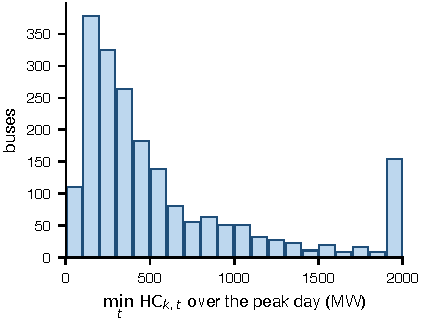
\includegraphics[width=\linewidth]{figures/hc_histogram.pdf}
    \end{column}
    \begin{column}{0.48\textwidth}
      \small
      ACTIVSg2000 synthetic Texas grid,\fcite{birchfield2017grid} 2028 Jul--Dec,
      the 24 hours of the peak-load day, all \HCbuses{} buses:
      \begin{itemize}
        \item smallest: \HCmin\MW
        \item median \HCmedian\MW
        % \item 10\% of buses below \HCpten\MW
        \item 90\% below \HCpninety\MW
        %  \HCabove{} buses above 2{,}000\MW{} (not shown)
      \end{itemize}
      \vspace{0.2em}
      % \HCruntime{} with \texttt{ercot-game-hosting-capacity} (Gurobi).
    \end{column}
  \end{columns}
\end{frame}

\begin{frame}{Over time: the stressed hours bind}
  \begin{columns}[T,onlytextwidth]
    \begin{column}{0.5\textwidth}
      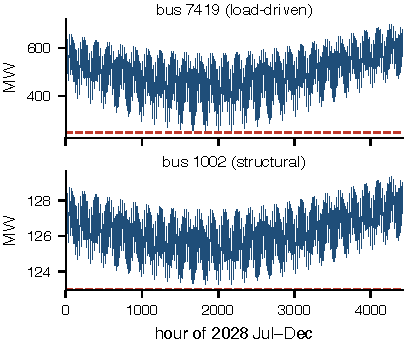
\includegraphics[width=\linewidth]{figures/hc_series.pdf}
    \end{column}
    \begin{column}{0.48\textwidth}
      \small
      A constant load must be served in \emph{every} hour:
      \[
        \keyeq{\HC_k = \min_t \HC_{k,t}}\quad\text{(dashed)}
      \]
      \begin{itemize}
        \item Bus \SerTwoBus: \SerTwoMin\MW{} to \SerTwoMax\MW, median
          \SerTwoMed\MW{}: tight at peak hours.
        \item Bus \SerOneBus: \SerOneMin\MW{} to \SerOneMax\MW{}: the network
          limits it, not the load cycle.
      \end{itemize}
      ``Dynamic hosting capacity'' treats this time variation
      explicitly.\fcite{deoliveira2019dynamic}
    \end{column}
  \end{columns}
\end{frame}

\begin{frame}{Many buses at once: the hosting-capacity region}
  \begin{columns}[T,onlytextwidth]
    \begin{column}{0.48\textwidth}
      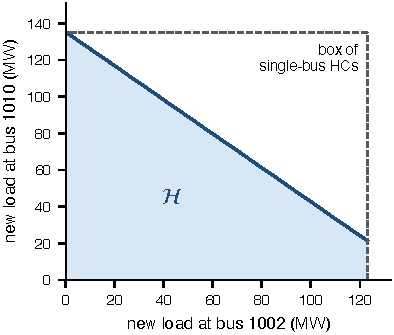
\includegraphics[width=\linewidth]{figures/hc_region.pdf}
    \end{column}
    \begin{column}{0.51\textwidth}
      \small
      The \alert{hosting-capacity region} $\mathcal H$: every combination of new
      loads $\mathbf x$ that the grid can serve in every hour.
      \begin{itemize}
        \item A convex polytope: the projection of the DCOPF feasible
          set.\fcite{gong2024adaptive}
        \item Single-bus HCs are its axis intercepts. They \alert{do not add
          up}.\fcite{wan2026hosting}
        \item Peak hour: bus 1002 hosts \PairHCa\MW{} alone, only
          \PairHCaGiven\MW{} with 60\MW{} at neighbor 1010.
      \end{itemize}
    \end{column}
  \end{columns}
\end{frame}

\begin{frame}{With a local generator}
  Site at bus $k$: load $\vL$, private gen $0\le \vg_t\le G$. The grid only
  sees the \emph{net} withdrawal $\vL-\vg_t$:
  \[
    \text{feasible} \iff 
    \pause
    \exists\, \vg_t\in[0,G]:\ \underbrace{\vL - \vg_t}_{\text{net withdrawal}} \le \HC_{k,t}\ \ \forall t
    \pause
    \quad\Longrightarrow\quad \keyeq{\HC_k^{G} = \min_t \HC_{k,t} + G}
  \]
  \begin{itemize}
    \item Exact when the generator is always available
    % ; with outages, ramping,
    %   or fuel limits, $\HC^G_k \le \HC_k + G$.
    \item The generator runs only when the grid is short or when its cost
      is below the local price.
    % \item Buying headroom: in the game \$1.5M per MW of generator, versus
    %   \$25M per MW of site that would otherwise go unserved.
  \end{itemize}
\end{frame}

\begin{frame}{Storage: move energy from slack hours to tight hours}
  \begin{columns}[T,onlytextwidth]
    \begin{column}{0.56\textwidth}
      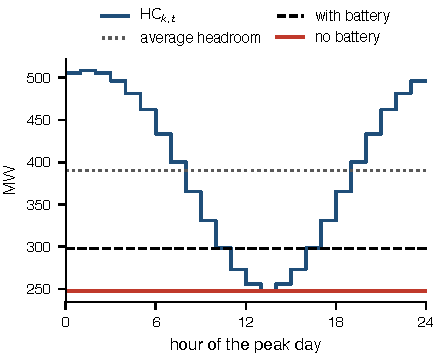
\includegraphics[width=\linewidth]{figures/storage_day.pdf}
    \end{column}
    \begin{column}{0.42\textwidth}
      \small
      Bus \StoBus, peak day, daily cycle\footnote{$\ve_0 = \ve_{24} = B/2$ and $B = 4P$}:
      \begin{itemize}
        \item no battery: \alert{\StoMin\MW}
        \item average headroom (dotted): \StoMean\MW{}, the most any battery could reach (next slide)
        \item $P = \StoP\MW$, $B = \StoB\MWh$: \alert{\StoWith\MW}
      \end{itemize}
      % $B$ limits how long a shortfall the battery can cover. Half-year:
      % \StoHalfNo{} $\to$ \StoHalfWith\MW.\\[0.2em]
    \end{column}
  \end{columns}
\end{frame}

\begin{frame}{With storage: the hours become coupled}
  \textbf{Battery at bus $k$}: power $P$, energy $B$, signed output $\vu_t$
  (positive = discharge), time step $\Delta t$; $\HC_{k,t}$ comes from the
  single-bus LP:
  \begin{align*}
    \HC_k^{S} = \max_{\vL,\,\vu,\,\ve}\ \vL \quad \text{s.t.}\quad
      & \underbrace{\vL - \vu_t \le \HC_{k,t}}_{\text{grid limit on net withdrawal}},
        \qquad \underbrace{-P \le \vu_t \le P}_{\text{power}},\\
      & \underbrace{\ve_t = \ve_{t-1} - \Delta t\, \vu_t,\quad 0 \le \ve_t \le B}_{\text{energy}},
        \qquad \underbrace{\ve_0 = \ve_T}_{\text{daily cycle}} .
  \end{align*}
  {\footnotesize Decision variables: $\vL$ new load, $\vu_t$ battery output,
  $\ve_t$ stored energy. A lossless battery (no round-trip losses)
  % , which makes
  % the bound below optimistic.
  }
  % \small
  \pause
  \begin{itemize}
    \item A multi-period LP: discharge in tight hours, recharge in slack
      ones.\fcite{macedo2017increasing}
    \item Summing over the cycle ($\sum_t \vu_t = 0$):
      $\keyeqin{\HC^S_k \le \frac1T \sum_t \HC_{k,t}}$: storage lifts the limit at
      most from the \alert{minimum} to the \alert{average} headroom.
      % ; power
      % ($\vL \le \HC_{k,t} + P$) and energy ($B$) keep it below that.
  \end{itemize}
\end{frame}


\begin{frame}{Flexibility: curtail in a few hours}
  \begin{columns}[T,onlytextwidth]
    \begin{column}{0.40\textwidth}
      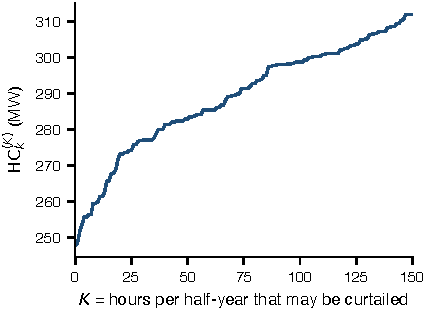
\includegraphics[width=\linewidth]{figures/order_statistic.pdf}
    \end{column}
    \begin{column}{0.59\textwidth}
      \footnotesize
      Flexible connection:\fcite{gu2026flexible}
      \[
        \begin{aligned}
          \max_{\vL,\,\vd}\ & \vL\\
          \text{s.t.}\ & \vL - \vd_t \le \HC_{k,t},\quad \vd\ge 0,\quad \|\vd\|_0 \le K
        \end{aligned}
      \]
      \begin{itemize}
        \item $\vd_t$ is the load curtailed in hour $t$; nonconvex ($\|\vd\|_0$ counts curtailed hours).
        \item $\keyeqin{\HC_k^{(K)} = \HC_{k,[K+1]}}$, the $(K{+}1)$-th \emph{smallest} hourly value.
        \item Bus \OrdBus:
        \begin{itemize}
          \item \OrdZero\MW{} at $K=0$,
          \item \OrdTwentyFour\MW{} at $K=24$ ($+$\OrdTwentyFourGain\%),
          \item \OrdHundred\MW{} at $K=100$ ($+$\OrdHundredGain\%).
        \end{itemize}
        % , 
        % ($+$\OrdTwentyFourGain\%), \OrdHundred\MW{} at $K=100$
        % ($+$\OrdHundredGain\%). Diminishing returns in $K$.\fcite{etherden2011increasing,sarker2026risk}
      \end{itemize}
    \end{column}
  \end{columns}
\end{frame}

\begin{frame}{How much should we trust a hosting-capacity number?}
  \begin{itemize}
    \item \textbf{Security.} Dropping N-1 contingencies overstates data-center
      hosting capacity by about 20\% on the IEEE RTS-24.\fcite{wan2026hosting}
    \item \textbf{Dynamics.} The data center's own ride-through limits (UPS,
      converters) can be the binding constraint.\fcite{ren2026ride}
    \item \textbf{Model.} DC power flow has no voltage or reactive-power limits
      and no losses.
    \item \textbf{Simultaneity.} Single-bus numbers ignore everyone else 
      connecting at the same time.
  \end{itemize}
  \pause
  \vspace{0.4em}
  The last point leads to the second question: \alert{who gets served?}
\end{frame}

% ===========================================================================
\section{Part II: The connection game}

\begin{frame}{From one bus to many applicants}
  \begin{columns}[c,onlytextwidth]
    \begin{column}{0.52\textwidth}
      \begin{itemize}
        \item Part I: one bus $\Rightarrow$ one number; many buses
          $\Rightarrow$ a \alert{region}.
        \item Two requests can each fit alone and still not fit together.
        \item Someone has to decide who is served, and by how much.
      \end{itemize}
      \vspace{0.8em}
      \alert{For the next three weeks, you are the applicants.}
    \end{column}
    \begin{column}{0.43\textwidth}
      \centering
      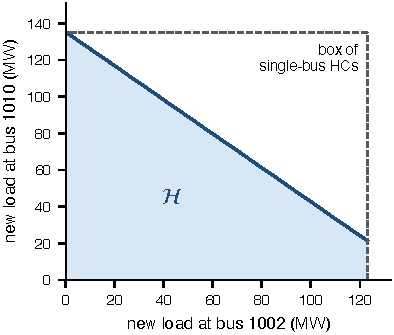
\includegraphics[width=\linewidth]{figures/hc_region.pdf}
    \end{column}
  \end{columns}
\end{frame}

\begin{frame}{Your role in one picture}
  \centering
  % One student site at a network bus: the data center, a private generator,
% and a battery, behind one grid connection. Needs fontawesome5 and the TikZ
% libraries positioning, calc, fit, shapes.misc.
\begin{tikzpicture}[font=\footnotesize, >=latex,
  icon/.style={font=\Huge},
  part/.style={draw, rounded corners=3pt, line width=0.8pt, minimum width=36mm,
    minimum height=13mm, inner sep=3pt, align=left},
  flow/.style={->, line width=1.1pt},
  bus/.style={circle, draw=ThemeDark, fill=white, line width=0.8pt, inner sep=1.6pt}]

  % The grid: a small mesh of buses.
  \foreach \n/\x/\y in {a/0/0, b/1.1/0.75, c/1.3/-0.7, d/2.3/0.15, e/0.25/1.25, f/0.15/-1.2} {
    \node[bus] (\n) at (\x,\y) {};
  }
  \foreach \u/\v in {a/b, a/c, b/d, c/d, a/e, e/b, a/f, f/c} {
    \draw[ThemeDark!70, line width=0.7pt] (\u) -- (\v);
  }
  \node[bus, fill=ThemeBlue!40, minimum size=5mm] (k) at (3.6,0.15) {$k$};
  \draw[ThemeDark!70, line width=0.7pt] (d) -- (k);
  \node[align=center, text=ThemeDark, below=4mm of c, xshift=4mm]
    {\textbf{the grid}\\joint DCOPF of all teams\\price $\lambda_{k,t}$ at bus $k$ at time $t$};

  % Your site.
  \node[part, draw=orange!80!black, fill=orange!8] (dc) at (8.3,0.15)
    {\begin{tabular}{@{}c@{\hspace{2mm}}l@{}}
      \textcolor{orange!80!black}{\Huge\faServer} &
      \begin{tabular}[c]{@{}l@{}}\textbf{Data center}, $C$\MW \end{tabular}
    \end{tabular}};
  \node[part, draw=green!50!black, fill=green!6, above=5mm of dc] (gen)
    {\begin{tabular}{@{}c@{\hspace{2mm}}l@{}}
      \textcolor{green!50!black}{\Huge\faIndustry} &
      \begin{tabular}[c]{@{}l@{}}\textbf{Generator}, $G \le C$ \end{tabular}
    \end{tabular}};
  \node[part, draw=violet!70!black, fill=violet!6, below=5mm of dc] (bat)
    {\begin{tabular}{@{}c@{\hspace{2mm}}l@{}}
      \textcolor{violet!70!black}{\Huge\faBatteryThreeQuarters} &
      \begin{tabular}[c]{@{}l@{}}\textbf{Battery}, $P$\MW, $B = 4P$\end{tabular}
    \end{tabular}};
  \node[draw=orange!80!black, dashed, rounded corners=5pt, line width=0.8pt,
    fit=(gen)(dc)(bat), inner xsep=10mm, inner ysep=3mm] (site) {};
  \node[anchor=south, text=orange!80!black, font=\footnotesize\bfseries]
    at (site.north) {your site = one row of the submitted CSV};

  % Flows.
  \draw[flow, ThemeDark] (k) -- node[above, align=center] {grid purchase\\(paid at $\lambda_{k,t}$)} (dc.west);
  \draw[flow, green!50!black] (gen.south) -- (dc.north);
  \draw[flow, violet!70!black, <->] (bat.north) -- (dc.south);
  \node[anchor=north, text=red!70!black, font=\scriptsize, align=center]
    at (site.south) {\faBan\ no export: the generator and battery serve only your own load};
\end{tikzpicture}
\\[0.3em]
  \small You choose the numbers $C$, $G$, $P$ for each site, and the grid operator
  runs them.
\end{frame}

\begin{frame}{What earns money, and when}
  \small
  One 50\MW{} site, planned on 5 representative days (120 hours) for 10 years:
  \begin{itemize}
    \item earns \alert{\$1{,}000 per MWh} served over ten years (7\% discount),
     costs \alert{\$25M per MW} (paid once).
    \item Energy is about \$18/MWh.
    % \item It breaks even at about \alert{41\% served}, so what matters is whether
    % the grid can deliver.
  \end{itemize}
  \centering
  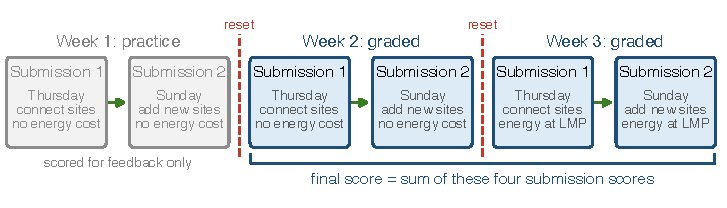
\includegraphics[width=\textwidth]{figures/timeline.pdf}\\[0.2em]
  % {\scriptsize Generator \$1.5M/MW; battery \$0.4M/MW $+$ \$0.25M/MWh; full table
  % in the tutorial.}
\end{frame}

\begin{frame}{What the grid operator does}
  % \small
  Part I's LP, with every team's \alert{submitted plans}:
  \begin{align*}
    \min\ & \text{generation cost} + \text{private generator cost}\\
    \text{s.t.}\ & \vp = M\vpg - \mathbf d_t - \text{(all teams' sites, net of their own generator and battery)},\\
    & \mathbf 1^{\top}\vp = 0,\quad \vf = \Phi\vp,\quad |\vf| \le \mathbf F,\quad
      \text{batteries' constraints.}
  \end{align*}
  \begin{itemize}
    \item One DCOPF per representative hour, coupled through the batteries over each day.
    \item The price of energy at your bus is the LMP.
    % \item The full LP is on the backup slide.
  \end{itemize}
\end{frame}

\begin{frame}{When it doesn't fit: how ERCOT connects large loads since 2026}
  \footnotesize
  \begin{columns}[T,onlytextwidth]
    \begin{column}{0.47\textwidth}
      \textbf{Before: one request at a time}
      \begin{itemize}
        \item Each new project could invalidate the studies of projects ahead of it.
        \item Repeated restudies and delays of years.
      \end{itemize}
      \pause
      \textbf{Now: a batch (PGRR145, ``Batch Zero'')}\fcite{ercot2026batch}
      \begin{itemize}
        \item All eligible loads are studied \alert{together}.
        \item Allocated ``based on what the grid can reliably support''.
        % \item Batch Zero allocations in spring 2027; Batch 1 opens summer 2027.
      \end{itemize}
    \end{column}
    % \pause
    \begin{column}{0.5\textwidth}
      % \textbf{Three kinds of applicant}
      % \begin{itemize}
      %   \item \textbf{Base load:} studied before and its MW are kept.
      %   \item \textbf{Studied load:} gets its full request, \alert{part of it}, or waits for the next batch.
      %   \item \textbf{Excluded:} waits for a future batch.
      % \end{itemize}
      \pause
      \textbf{Minimum allocation}\fcite{ercot2026pgrr145}
      \begin{itemize}
        \item Request above 100\MW: an allocation below \alert{100\MW} is
          \alert{reduced to zero}.
        \item Request of 100\MW{} or less: an allocation below \alert{90\%}
          of the request is \alert{reduced to zero}.
      \end{itemize}
      \textbf{Ways to connect sooner}
      \begin{itemize}
        \item Bring your own generation, or let ERCOT curtail you under stress (Part I).
      \end{itemize}
    \end{column}
  \end{columns}
\end{frame}

\begin{frame}{The game's batch rule: one shared limit}
  \small
  Three teams behind one line that can carry \alert{200\MW{}} of new load.
  \\Requests: A 40, B 100, C 200 (total 340).
  \begin{columns}[T,onlytextwidth]
    \begin{column}{0.58\textwidth}
      \begin{enumerate}
        \item<2-> \textbf{Common level.} Raise $t$ until the line is full:
          $\min(40,t)+\min(100,t)+\min(200,t)=200 \Rightarrow t = 80$.\\
          \alert{A gets 40 (all), B 80, C 80.}
        \item<3-> \textbf{Minimum allocation.} C gets $80/200 = 40\% < 50\%$
          $\Rightarrow$ C is dropped (largest short request first).
        \item<4-> \textbf{Recompute without C.} $40 + 100 = 140 \le 200$:
          A and B are served in full.
      \end{enumerate}
    \end{column}
    \begin{column}{0.41\textwidth}
      \centering
      \begin{tabular}{@{}lrrr@{}}
        \toprule
        & request & \only<1-3>{step 1}\only<4->{final} & share\\
        \midrule
        A & 40 & 40 & \only<1-3>{100\%}\only<4->{100\%}\\
        B & 100 & \only<1-3>{80}\only<4->{100} & \only<1-3>{80\%}\only<4->{100\%}\\
        C & 200 & \only<1-3>{80}\only<4->{\alert{0}} & \only<1-3>{40\%}\only<4->{\alert{0\%}}\\
        \bottomrule
      \end{tabular}\\[0.8em]
      \onslide<5->{\footnotesize C still pays capital on 200\MW{}.
      \alert{Asking for more than the grid can give is the most expensive mistake in the game.}}
    \end{column}
  \end{columns}
  \vspace{0.6em}
  \onslide<5->{\footnotesize ERCOT does not publish a formula for splitting capacity among
  studied loads. The game uses \alert{equal MW} (the uniform
  rule\fcite{sprumont1991division}) so that everyone can predict it.}
\end{frame}

\begin{frame}{On the network: sharing the region}
  \small
  \centering
  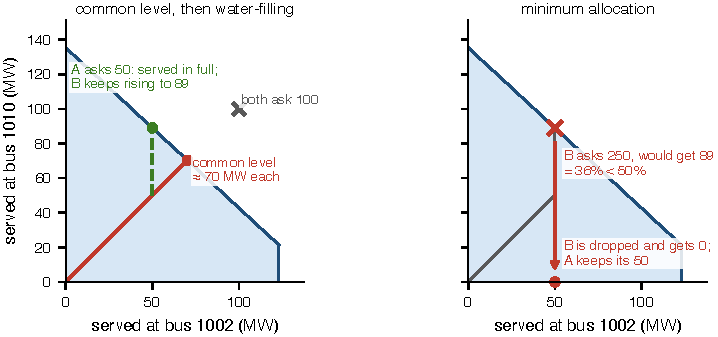
\includegraphics[width=0.7\textwidth]{figures/region_sharing.pdf}
  \begin{enumerate}
    \item Everyone rises to a \alert{common MW level}. A team that asked for less is served in full.
    \item Teams that are not blocked keep rising (water-filling).
    \item A team that would get \alert{less than half} of its request gets nothing.
  \end{enumerate}
\end{frame}

% \begin{frame}{The game and ERCOT}
%   \small
%   \begin{tabular}{@{}>{\raggedright\arraybackslash}p{0.24\textwidth}>{\raggedright\arraybackslash}p{0.36\textwidth}>{\raggedright\arraybackslash}p{0.34\textwidth}@{}}
%     \toprule
%     & ERCOT batch study & This game\\
%     \midrule
%     Who is studied together & All eligible loads in a batch & All teams' submissions\\
%     Already connected & Base load keeps its MW & \texttt{ACTIVSg2000}'s existing load\\
%     How MW are split & System-wide study & Equal MW level, then water-filling\\
%     Too small a share & below 100\MW{} (90\% for requests $\le$100\MW) $\to$ 0 & below 50\% of the request $\to$ 0\\
%     Commitment & Financial security, site control & Capital charged on the full request\\
%     Own generation & Offsets transmission need & Private generator $G$\\
%     Flexible load & May be curtailed under stress & Not in the game (Part I)\\
%     \bottomrule
%   \end{tabular}\\[0.8em]
%   % The 50\% threshold is scaled to the game's 50--200\MW{} requests; ERCOT's
%   % 100\MW{} floor would drop almost every team.
% \end{frame}

\begin{frame}{A two-team example}
  \small
  Team A at bus 1002, team B at neighbor 1010; each picks 50 or 100\MW{} in Submission 1.\\[0.3em]
  Ten-year payoffs, Weeks 1--2 (\$M), A's payoff / B's payoff:
  \begin{center}
    \begin{tabular}{@{}lcc@{}}
      \toprule
      A \textbackslash{} B & B small (50) & B large (100)\\
      \midrule
      A small (50) & 1,826 / 1,826 & \only<2->{\fbox{\textbf{1,826}} / \fbox{\textbf{2,980}}}\only<1>{1,826 / 2,980}\\
      A large (100) & \only<2->{\fbox{\textbf{3,172}} / \fbox{\textbf{1,826}}}\only<1>{3,172 / 1,826} & 1,820 / 1,820\\
      \bottomrule
    \end{tabular}\\[0.3em]
    \onslide<2->{\scriptsize Boxed: each team's best response to the other's choice.
    A cell with both boxed is a Nash equilibrium.}
  \end{center}
  \begin{itemize}
    \item<2-> If B goes small, A should go large. If B goes large, A should go small.
    \item<3-> Nash equilibria: (A small, B large); (A large, B small). 
    % A game of
    %   \emph{chicken}: if both insist, both lose. In Week 3, congestion adds
    %   \$400--770M of energy cost per team.
    \item<4-> Your score depends on where everyone builds, and you see the results
      between submissions. \alert{What would you do?}
  \end{itemize}
\end{frame}

% \begin{frame}{From the slides to your laptop}
%   \centering
%   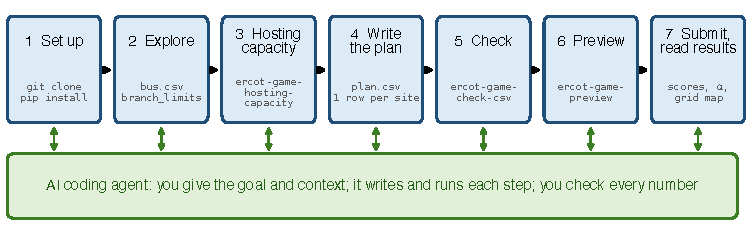
\includegraphics[width=\textwidth]{figures/workflow.pdf}\\[0.6em]
%   \small Everything is in one GitHub repository: \hyperlink{https://github.com/MhaoMou/ercot-connection-planning-instructor}{\alert{[Link]}}.\\[0.3em]
%   The tutorial walks through a full session with an AI coding agent on a 14-bus demo.\\
%   % The tutorial's Part I is the official assignment; Part II walks through every step.
% \end{frame}



\begin{frame}{After each round, and your first plan}
  \small
  \begin{columns}[T,onlytextwidth]
    \begin{column}{0.5\textwidth}
      \textbf{What you get back}
      \begin{itemize}
        \item your score breakdown (in private);
        \item every team's service fraction $\alpha$\%;
        \item a grid map with the total MW at each bus.
      \end{itemize}
      \textbf{A first plan for Week 1}
      \begin{enumerate}
        \item Shortlist buses by hosting capacity.
        \item Ask well below it if w/o a generator or battery.
        \item Check, preview, change one thing, compare.
      \end{enumerate}
    \end{column}
    \begin{column}{0.48\textwidth}
      \centering
      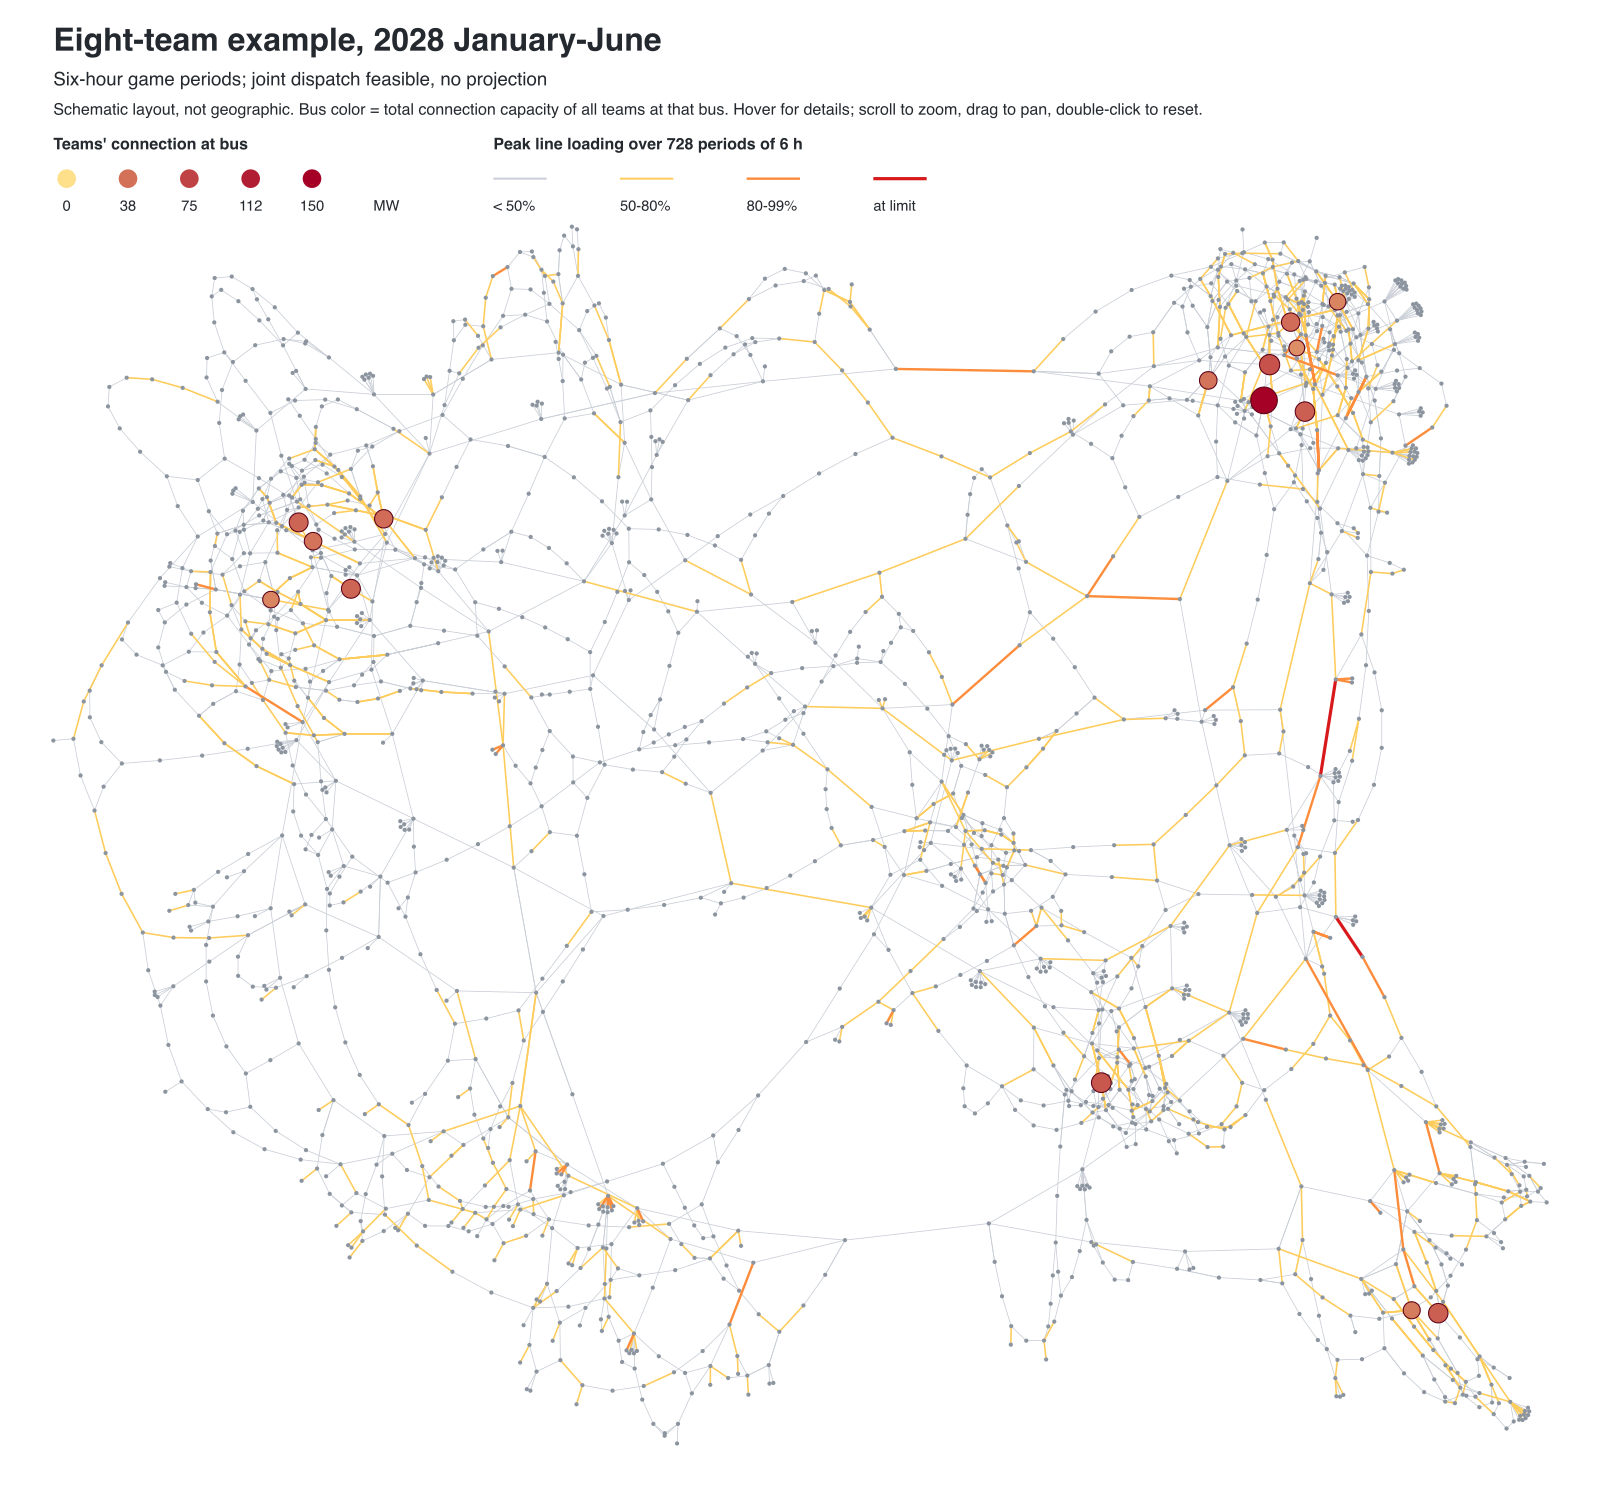
\includegraphics[width=0.78\linewidth]{figures/grid_map.png}\\[-0.2em]
      {\scriptsize Eight-team example: bus color = total MW of all teams,
      line color = peak loading; approximate locations.}
    \end{column}
  \end{columns}
\end{frame}

\begin{frame}{Takeaways}
  \begin{itemize}
    \item Hosting capacity is an LP: the DCOPF with a ``maximize the new load''
      objective.
    \item Time: a constant load is limited by the \alert{worst} hour.
      Generation adds $G$ and storage moves the limit toward the
      \alert{average}. Flexibility toward the $(K{+}1)$-th worst.
    \item Space: single-bus numbers are intercepts of a region and
      \alert{do not add up}.
    \item With many applicants, \alert{who gets served} is a design choice, and it turns planning
      into a \alert{game}.
  \end{itemize}
  \vspace{0.6em}
  \textbf{Questions for you.} How should a grid operator allocate scarce headroom
  among data centers? What would you change in the game's rule?
\end{frame}

\begin{frame}[allowframebreaks]{References}
  \printbibliography[heading=none]
\end{frame}


\appendix
\begin{frame}{Backup: the evaluator in full}
  \small
  For each representative day $d = 1,\dots,5$ and hour $t = 1,\dots,24$
  ($\Delta t = 1$\,h, 120 hours in all): a DCOPF with all teams' sites, coupled
  within each day through batteries and generator run-hour budgets.
  \begin{align*}
    \min\ & \textstyle\sum_{d,t} \Delta t \big(\mathbf c^{\top}\vpg[dt] + \sum_s \sum_m c^m q^m_{s,dt}\big)\\
    \text{s.t.}\ & \text{DCOPF balance and line limits with loads } \alpha_i C_s
      \text{ and private } q_s, \vu_s\\
    & \ve_{s,d,t} = \ve_{s,d,t-1} - \Delta t\, \vu_{s,dt},\ \ 0\le \ve\le B_s,\ \ |\vu|\le P_s,\ \
      \ve_{s,d,0} = \ve_{s,d,24} = B_s/2\\
    & \textstyle\sum_{t,m} \Delta t\, q^m_{s,dt} \le h\, G_s \quad\text{(generator run-hour budget, } h = 2\text{ h per day)}\\
    & \textstyle\sum_{s\in i,\,k(s)=n} \vu_{s,dt} \le \sum_{s\in i,\,k(s)=n} \alpha_i C_s
      \quad\text{(a team's assets serve only its own load)}
  \end{align*}
  \begin{itemize}
    \item An exact LP that separates by day (Benders or one LP per day).
    \item LMP = dual of nodal balance; it prices energy in Week 3.
    \item Scores weight each hour by the days it stands for, over ten years in present value.
  \end{itemize}
\end{frame}

\begin{frame}{Backup: the hosting-capacity region}
  The single-bus LP's constraints with new loads $\mathbf x$ (one per bus) in
  place of $\vL\,\mathbf e_k$:
  \[
    \mathcal H = \left\{\mathbf x \ge 0 :\
    \begin{aligned}
      &\forall t\ \exists\, \vpg[t], \vp_t:\\
      &\vp_t = M\,\vpg[t] - \mathbf d_t - \mathbf x,\ \ \mathbf 1^{\top}\vp_t = 0,\\
      &|\Phi\vp_t| \le \mathbf F,\ \ \mathbf p^{\min} \le \vpg[t] \le \mathbf p^{\max}
    \end{aligned}\right\}
  \]
  A convex polytope: the projection of the DCOPF feasible set onto the new
  loads. The single-bus hosting capacity $\HC_k$ is its intercept on axis $k$.
\end{frame}

\end{document}
